\section{Introduction}
% Computer Society journal papers do something a tad strange with the very
% first section heading (almost always called "Introduction"). They place it
% ABOVE the main text! IEEEtran.cls currently does not do this for you.
% However, You can achieve this effect by making LaTeX jump through some
% hoops via something like:
%
%\ifCLASSOPTIONcompsoc
%  \noindent\raisebox{2\baselineskip}[0pt][0pt]%
%  {\parbox{\columnwidth}{\section{Introduction}\label{sec:introduction}%
%  \global\everypar=\everypar}}%
%  \vspace{-1\baselineskip}\vspace{-\parskip}\par
%\else
%  \section{Introduction}\label{sec:introduction}\par
%\fi
%
% Admittedly, this is a hack and may well be fragile, but seems to do the
% trick for me. Note the need to keep any \label that may be used right
% after \section in the above as the hack puts \section within a raised box.



% The very first letter is a 2 line initial drop letter followed
% by the rest of the first word in caps (small caps for compsoc).
% 
% form to use if the first word consists of a single letter:
% \IEEEPARstart{A}{demo} file is ....
% 
% form to use if you need the single drop letter followed by
% normal text (unknown if ever used by IEEE):
% \IEEEPARstart{A}{}demo file is ....
% 
% Some journals put the first two words in caps:
% \IEEEPARstart{T}{his demo} file is ....
% 
% Here we have the typical use of a "T" for an initial drop letter
% and "HIS" in caps to complete the first word.
\IEEEPARstart{F}{REEDM} (Future Renewable Electric Energy Delivery and Management) is a smart grid project focused on the future of the electrical grid.
Major proposed features of the FREEDM network include the solid state transformer, distributed local energy storage, and distributed local energy generation \cite{FREEDMMIGRATION}.
This vein of research emphasizes decentralizing the power grid, making it more reliable by distributing energy production resources.
Part of this design requires the system to operate in islanded mode, where portions of the distribution
network are segmented from each other.

The effects of these partitions are still not well understood.
This is particularly true in a distributed cyber-physical system, in which partitions may occur in both the cyber and physical domains.
As a result,it is not well known how either a cyber or physical faults will effect the other portion of the system.
However, previously conducted research \cite{HARINI}\cite{TSG} indicates that cyber faults can cause a
physical system to apply unstable settings.

This work presents the initial steps neccessary to better understanding and planning for these faults.
A new approach to considering how a distributed system interacts during a fault condition allows for the creation of new techniques for managing a fault scenario in cyber-physical systems. 
This discussion presents an approach that utilizes Markov chain to model a system's grouping behavior.
These chains produce expectations with regard to not only how long a system can be expected to stay in a particular state but also much time it will be able to spend coordinating and doing useful work over a period
of time. 
Using these measures, the behavior of the control system for the physical devices can be adjusted to prevent faults.

The next section describes both the FREEDM smart-grid system and it's Distributed Grid Intelligence (DGI).
Section 3, includes an overview the group management algorithm, and the state of the art for distributed systems.
Section 4 discusses the architecture of the DGI, including the architecture of the message passing interface and the protocols used in the experiments, and the experimental setup.
Section 5 outlines previously gathered results collected by running the DGI in a controlled environment.
Section 6 explains the assumptions made and the Markov Chain's construction. 
Section 7 focuses on the accuracy of these models for predicting grouping behavior.
Section 8 offers summary and conclusion.

%\IEEEpubidadjcol
% needed in second column of first page if using \IEEEpubid
\section{FREEDM DGI}
This models the group management module of the FREEDM DGI.
The DGI is a smart grid operating system that organizes and coordinates power electronics.
It also negotiates contracts to deliver power to devices and regions that cannot effectively facilitate their own needs.
DGI leverages common distributed algorithms to control the power grid, making it an attractive target for modeling a distributed system.

The DGI software consists of a central component, known as the broker.
This broker is responsible for presenting a communication interface.
It also furnishes any common functionality the system's algorithms may need.
These algorithms, grouped into modules, work in concert to move power from areas of excess supply to excess demand.

DGI utilizes several modules to manage a distributed smart-grid system.
Group management, the focus of this work, implements a leader election algorithm to discover which processes are reachable within the cyber domain.
Other modules provide additional functionality, such as collecting global snapshots, negotiating the migrations, and giving commands to physical components.

DGI is a real-time system; certain actions (and reactions) involving power system components need to be completed within a pre-specified time-frame to keep the system stable.
It uses a round robin schedulerin which each module is given a predetermined window of execution which it may use to perform its duties.
When a module's time period expires, the next module in the line is allowed to execute. 
 
\section{Group Management}
The DGI uses the leader election algorithm, ``Invitation Election Algorithm,'' written by Garcia-Molina \cite{INVITATIONELECTION}.
Originally published in 1982, this algorithm provides a robust election  procedure that allows for transient partitions.
Transient partitions are formed when a faulty link between two or more clusters of DGIs causes the groups to divide temporarily.
These transient partitions merge when the link becomes more reliable.
The election algorithm allows for failures that disconnect two distinct sub-networks.
These sub networks are fully connected, but connectivity between the two sub-networks is limited by an unreliable link.

Since Garcia-Molina's original publication \cite{INVITATIONELECTION}, a large number of election algorithms have been created. 
Each algorithm is designed to be well-suited to the circumstances it will deployed in.
Specialized algorithms exist for wireless sensor networks \cite{LE-WSN-1}\cite{LE-WSN-2}, detecting failures in certain circumstances \cite{LE-SPECIALCIRCUMSTANCES-1}\cite{LE-SPECIALCIRCUMSTANCES-2}, and of course, transient partitions.
Work on leader elections has been incorporated into a variety of distributed frameworks: Isis \cite{ISISTOOLKIT}, Horus \cite{HORUSTOOLKIT}, Totem \cite{TOTEMTOOLKIT}, Transis \cite{TRANSISTOOLKIT}, and Spread \cite{SPREADTOOLKIT} all have methods for creating groups.
Despite this wide array of work, the fundamentals of leader election are consistent
across all work.
Processes arrive at a consensus of a single peer that coordinates the group.
Processes that fail are detected and removed from the group. 

The elected leader is responsible for making work assignments, and identifying and merging with other coordinators when they are found, as well as maintaining an up-to-date list of peers for the members of his group. 
Group members monitor the group leader by periodically checking if the group leader is still alive by sending a message. 
If the leader fails to respond, the querying nodes will enter a recovery state and operate alone until
they can identify another coordinator.
Therefore, a leader and each of the members maintain a set of processes which are currently reachable, a subset of all known processes in the system.

Leader election can also be classified as a failure detector \cite{LEADERELECTIONEVAL}.
Failure detectors are algorithms which detect the failure of processes within a system; they maintain a list of processes that they suspect have crashed.
This informal description gives the failure detector strong ties to the leader election process. 
The group management module maintains a list of suspected processes which can be determined from the set of all processes and the current membership.

The leader and the members have separate roles to play in the failure detection process.
Leaders use a periodic search to locate other leaders in order to merge groups.
This serves as a ping / response query for detecting failures within the system.
The member sends a query its leader.
The member will only suspect the leader, and not the other processes in their group.
Of course, simple modifications could allow the member to suspect other members.
However, that modification is not implemented in DGI code.

In this work it is assumed that a leader does not span two partitioned networks; if a group was able to form, all members have some chance of communicating with one another.

We define a metric to assess the performance of the system under duress.
A distributed can only perform meaningful work when the processes can work together to perform physical migration.
This means that there are two networks that affect the system's ability to do work: the physical flow network and the cyber communication network.

\section {Experimental Setup}

\subsection{Broker Architecture}
The DGI software used in this designed around a broker architectural specification.
Each core functionality of the system was implemented within a module that was provided access to core interfaces.
These interfaces provided functionality such as scheduling requests, message passing, and a framework to manipulate physical devices.

The Broker provided a common message passing interface that all modules could access.
This interface was then used to pass information between modules. 
For example, the list of peers in the group was sent as a message. 

Several of the distributed algorithms used in the software required the use of ordered communication channels.
DGI provided a reliable ordered communication protocol (The sequenced reliable connection or SRC).
It also offered a ``best effort'' protocol (The sequenced unreliable connection or SUC).
This protocol was also FIFO (first in, first out), but provided limited delivery guarantees.

Simple message delivery schemes were used in order to avoid complexities introduced by using TCP.
Constructing a TCP connection to a process that either had failed or was unreachable required a considerable amount of time.
We elected to use UDP packets which do not have those issues, since the protocol is connectionless.
UDP also allowed for the development of multiple protocols with various properties to evaluate which properties are desirable.
Lightweight protocols which were best effort oriented were implemented to deliver messages within the requirements.
The protocols listed here continued operating despite omission failures.
They follow the assumption that not every message is critical to the operation of the DGI and that the channel did not need to halt entirely to deliver one of the messages.

\subsection{Sequenced Reliable Connection}
The sequenced reliable connection was a modified send and wait protocol that had the ability to stop resending messages and move on to the next one in the queue if the message delivery time exceeded some timeout. 
The design of this protocol met several criteria:

\begin{itemize}
\item Messages needed to be delivered in order. A number of distributed algorithms rely on the assumption that the underlying message channel is FIFO.
\item Messages could become irrelevant.
Some messages may only have a short period in which they are worth sending. 
Beyond that time period, they should be considered inconsequential and thus, skipped.
Message expiration times were used to address this issue.
After a certain amount of time had passed, the sender would longer attempt to write that message to the channel.
Instead, he would proceed to the next unexpired message and attach a ``kill'' value. 
The kill value was the sequence number of the last message the sender knows the receiver accepted.
\item Every effort needed to be made to deliver a message while it was still relevant.
\end{itemize}

One adjustable parameter, the resend time, controlled how often the system would attempt to deliver a message it had not received an acknowledgment for.
A resend function was periodically called in an attempt to redeliver lost messages to the receiver.

\subsection{Sequenced Unreliable Connection}
The SUC protocol was a best effort protocol: it employed a sliding window to deliver messages as quickly as possible.
A window size was chosen, the sender can have up to that many outstanding messages at any given time.
The receiver would look for increasing sequence numbers, and disregard any message that was of a lower sequence number than was expected.
The purpose of this protocol was to implement a bare minimum: messages were accepted in the order they are sent.

The SUC protocol's resend time could be adjusted. 
Additionally, the window size was configurable. 
However the window size was left unchanged for the tests presented in this work.

The SUC protocol was developed because early hypothesis omission failures supposed that a lighter weight protocol might be more advantageous.
The lightweight protocol also presented a more complex behavior to model using Markov chains, since the nature of the protocol allowed for a race condition were a packet is lost.

\subsection{Experimental Setup}
Network unreliability was simulated by dropping datagrams from specific sources on the receiver side.
Each receiver was given an XML file describing the prescribed reliability of messages arriving from a specific source.
The network settings were loaded at run time and could be polled if necessary for changes in the link reliability.

``Lost'' messages are dropped on the receiver side. 
Code was inserted in the datagram processing code of the broker.
The broker would not deliver the message to the modules if the message is selected to be dropped.
On receipt of a message, the broker's examinesdthe source and randomly selected based on the prescribed reliability to drop a message.
A dropped message was not delivered to any of the modules and was not acknowledged by the receiver.
This method emulated a lossy network link but not one with message delays.

\section{Previous Results}
Initial data was collected from a non-real time version of the DGI code.
For each selected message arrival chance, as many as forty tests were run.
The collected results from the tests are divided into several target scenarios as well as the protocol used.

The first minute of each test in the experimental test is discarded so that any transients in the test could be removed.
The tests were run for ten minutes, however the maximum result was 9 minutes of in group time.
These graphs first appeared in \cite{CRITIS2012}.

\subsection{Sequenced Reliable Connection}

\subsubsection{Two Node Case}

The 100ms resend SRC test with two nodes can be considered a type of control in this study.
These tests, pictured in Figure \ref{fig:IGT-SRC-2NODE-100}, highlight the performance of the SRC protocol.
The maximum in group time of 9 minutes was achieved with only 15\% of datagrams arriving at the receiver. 

\begin{figure}[!h]
\centering
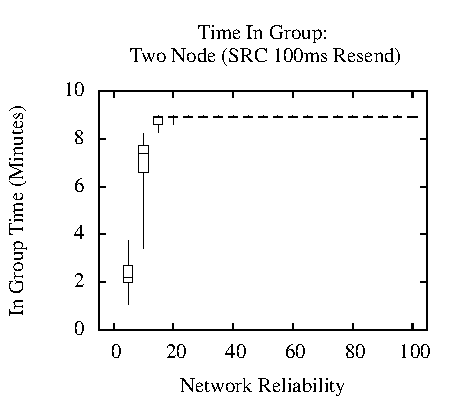
\includegraphics[width=\linewidth]{2NODE-SRC-100-GROUP.pdf}
\caption{Time in-group over a 10 minute run for a two node-system with a 100ms resend time}
\label{fig:IGT-SRC-2NODE-100}
\end{figure}

\begin{figure}[!h]
\centering
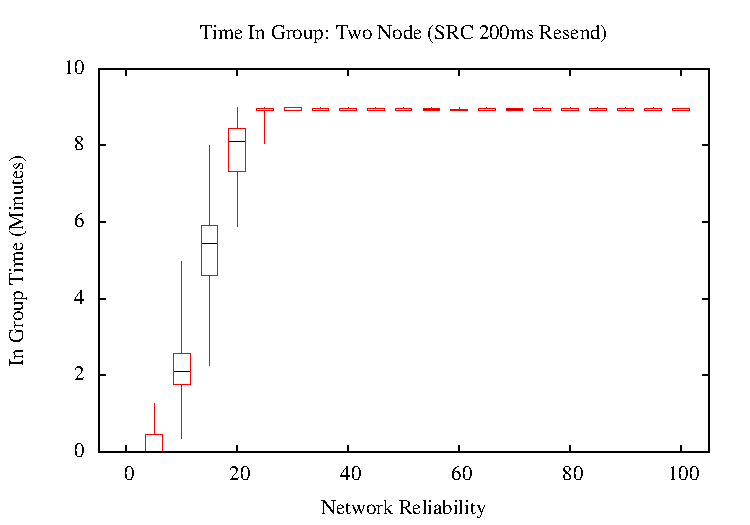
\includegraphics[width=\linewidth]{2NODE-SRC-200-GROUP.pdf}
\caption{Time in-group over a 10 minute run for a two node-system with a 200ms resend time}
\label{fig:IGT-SRC-2NODE-200}
\end{figure}

Figure \ref{fig:IGT-SRC-2NODE-200} demonstrates that as the rate at which lost datagrams were re-sent was decreased to 200ms, the in-group time decreased.
This behavior was expected.
Each exchange had a time limit for each message to arrive and the number of attempts was reduced by increasing the resend time.

\subsubsection{Transient Partition Case}

\begin{figure}[!h]
\centering
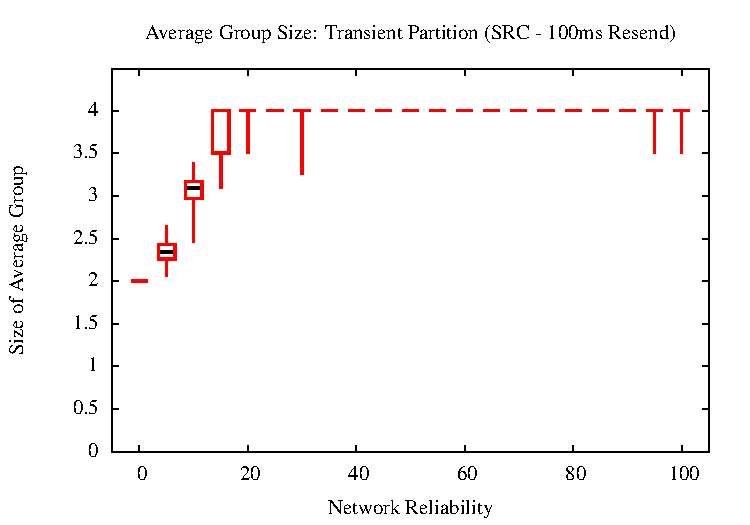
\includegraphics[width=\linewidth]{TRANS-SRC-100-SIZE.pdf}
\caption{Average size of formed groups for a transient partition case with a 100ms resend time}
\label{fig:MGS-SRC-TRANS-100}
\end{figure}

\begin{figure}[!h]
\centering
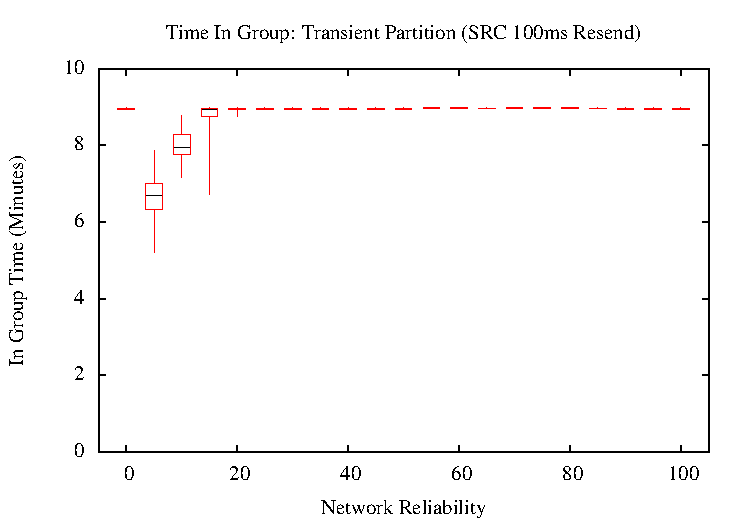
\includegraphics[width=\linewidth]{TRANS-SRC-100-GROUP.pdf}
\caption{Time in-group over a 10 minute run for a transient partition case with a 100ms resend time}
\label{fig:IGT-SRC-TRANS-100}
\end{figure}

The transient partition case is a simple example in which a network partition separates two groups of DGI processes. In the simplest case where the opposite side of the partition is unreachable, nodes will form a group with the other nodes on the same side of the partition.
In this study, two processes were present on each side of the partition.
In the experiment, the probability of a datagram crossing the partition was increased as the experiment continued.
The 100ms case is shown in Figures \ref{fig:MGS-SRC-TRANS-100} and \ref{fig:IGT-SRC-TRANS-100}.

While messages cannot cross the partition, the DGIs stay in a group with the nodes on the same side of the partition, leading to an in-group time of 9 minutes (the maximum value possible).
As packets began to cross the partition (as the reliability increases), DGI instances on either side attempted to complete elections with the nodes on the opposite partition and the in group time began to decrease.
During this time, however, the mean group size continued to increase.
Thus, while the elections were decreasing the amount of time that the module spent in a state where it can actively do work, it typically did not fall into a state where it was in a group by itself. 
As result, most of the lost in group time comes from elections.

\begin{figure}[!h]
\centering
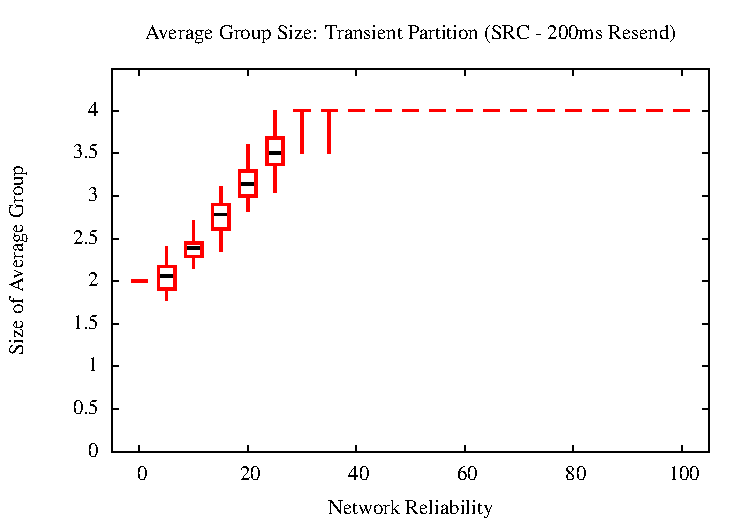
\includegraphics[width=\linewidth]{TRANS-SRC-200-SIZE.pdf}
\caption{Average size of formed groups for a transient partition case with a 200ms resend time}
\label{fig:MGS-SRC-TRANS-200}
\end{figure}

\begin{figure}[!h]
\centering
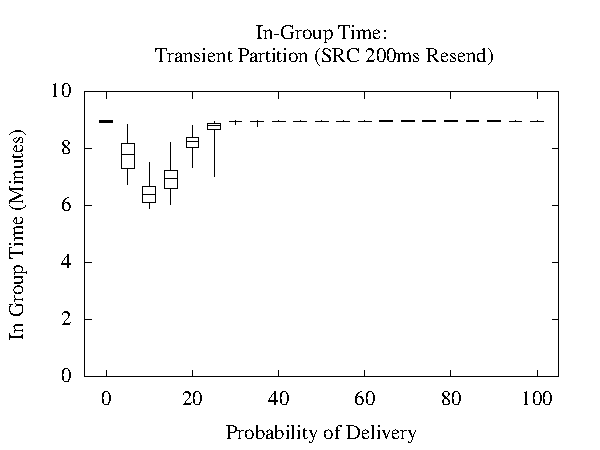
\includegraphics[width=\linewidth]{TRANS-SRC-200-GROUP.pdf}
\caption{Time in-group over a 10 minute run for a transient partition case with a 200ms resend time}
\label{fig:IGT-SRC-TRANS-200}
\end{figure}

The 200ms case (Illustrated in Figures \ref{fig:MGS-SRC-TRANS-200} and \ref{fig:IGT-SRC-TRANS-200}) suggests a similar behavior to Figures \ref{fig:MGS-SRC-TRANS-100} and \ref{fig:IGT-SRC-TRANS-100}, with a wider valley produced by the reduced number of datagrams.
The mean group size dips below 2 in Figure \ref{fig:MGS-SRC-TRANS-200}, possibly because longer resend times allowed for a greater number race conditions between potential leaders.
Discussion of these race conditions is shown and discussed during the SUC section since it was more prevalent in those experiments.

\subsection{Sequenced Unreliable Connection}

\subsubsection{Two Node Case}

The SUC protocol's experimental tests revealed an immediate problem.
There is a general increasing trend for the amount of time in-group shown in Figure \ref{fig:IGT-SUC-2NODE-100}.
There is a high amount of variance, however, for any particular trial.

\begin{figure}[!h]
\centering
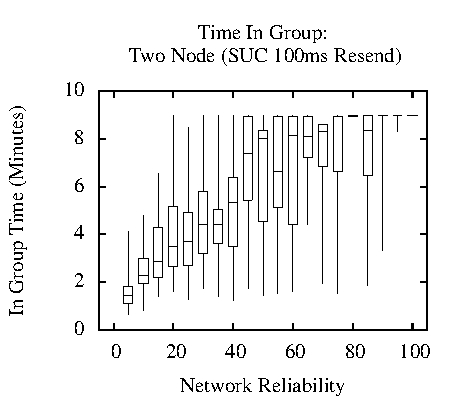
\includegraphics[width=\linewidth]{2NODE-SUC-100-GROUP.pdf}
\caption{Time in-group over a 10 minute run for a two node system with a 100ms resend time}
\label{fig:IGT-SUC-2NODE-100}
\end{figure}

\begin{figure}[!h]
\centering
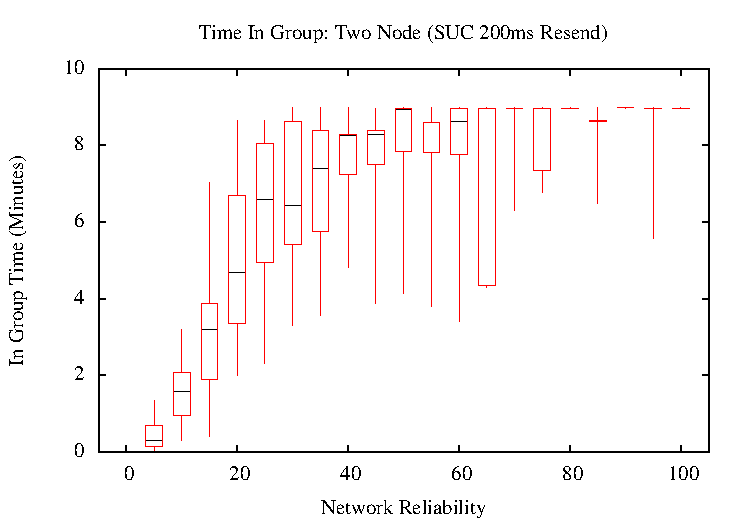
\includegraphics[width=\linewidth]{2NODE-SUC-200-GROUP.pdf}
\caption{Time in-group over a 10 minute run for a two node system with a 200ms resend time}
\label{fig:IGT-SUC-2NODE-200}
\end{figure}

In the 200ms resend case (illustrated in Figure \ref{fig:IGT-SUC-2NODE-200}), a greater growth rate occured in the in group time as the reliability increased.
When an average was taken across all of the collected data points from the experiment, the average in group time is higher for the 200ms case than it was for the 100ms case (6.86 vs 6.09).
There large amount of variance in the collected in group time, however.
As a result, it is not possible to state with confidence that the there is a significant difference between the two cases.

\section{Formal Modeling}

As a consequence of the high amount of variance in the collected data, it is difficult to make any predictions about other configurations from the collected data.
The behavior of the DGIs acting togethere was be modeled as a collection of states.
Each state described configuration of the system, and that the transitions between those states model failure events or election events.
These transitionas are probabilistic, and as a result it is a natural extension to model the distributed system as a Markov Chain.

\subsection{Assumptions}
The inter-arrival time between events was assumed to be exponentially distributed.
Furthermore, it was assumed that the system would be relatively well synchronized, with most elections occurring at the same time.
This assumption was valid for the 2-node cases in the non-real-time code. 
An increased number of processes violated this assumption for the non-real-time code.
With the use of the round-robin scheduler with synchronization it was possible enforce the synchronization assumption with the real-time code.

All participating peers were assumed to be on the same schedule; all peers began executing the model simultaneously.
Synchronization was accomplished using Choi's work \cite{DCS}.
It was also assumed the clocks are synchronized. 
If the network has faulted, process clocks would not drift noticeably from their last synchronization.
A production system would likely use GPS time synchronization to obtain certain power system readings \cite{PHASORREADINGS}.

\subsection{Constructing The Markov Chain}

Consider a set of processes, that are linked by some packet-based network protocol.
Under ideal conditions, a packet sent by one process  will always be delivered to its destination.
Without a delivery protocol, as soon as packets are lost by the communication network, the message that it contained is lost forever.
Therefore to compensate for packet loss, a large variety of delivery protocols have been developed.
Each protocol has a different set of goals and objectives, dependent on the application.
Two protocols, each with different delivery characteristics, were used in this study.

A single lost packet does not necessitate that the message it contained is forever lost.
Different protocols allow for different levels of reliability, despite packet loss.

The leader election algorithm was centered around two critical events: checking and elections.
The check system is used to detect both crash-stop failures and the availability of processses for election.
Processes in the system occasionally exchanged messages to determine if the other processes had failed.
Leaders exchanged messages to discover new leaders. 

The DGI could perform work if in a group, and not in an election state. 
The group management module instructs other modules to stop during an election.
The collected data in the previous sections was based on that assumption.
The Markov chains that model those scenarios also use that assumption.

Events in the distributed system were assumed to be distributed exponentially.
These were modeled in the chain by $\lambda(x)$ the parameter of the exponential distribution.
It is important to note that
\begin{equation}
\mathrm{E}[X] = \frac{1}{\lambda}. \!
\end{equation}
\begin{equation}
\lambda(x) = \sum \lambda(x,y) = \sum \lambda(x) p(x,y)
\end{equation}
where $\lambda(x)$ is the exponential parameter for the total time spent in a state $x$, $\lambda(x,y)$ is the exponential parameter for a transition from state $x$ to state $y$, and $p(x,y)$ is the normally distributed probability of transitioning from state $x$ to state $y$.

\subsubsection{Failure Detection}
When a leader sent its check messages, the processes either responded in the positive (indicating that they are also leaders) or in the
negative (indicating that they have already joined a group).
This message was sent to all known nodes in the system.
If a process replied that it was also a leader, the original sender entered an election mode and attempted to combine groups with the first process.
Members that failed to respond were removed from the leader's group.

In contrast, the member only sent a check message to the leader of its current group.
As with the leader's check message, the response could be either positive or negative.
A ``yes'' response indicated that the leader is still available and considered the member a part of its group.
A ``no'' response indicated that either the leader had failed and recovered, or it has suspected the member process of being unreachable.
In either case, the member had been removed from the leader's group.
The member would enter a recovery state and reset itself to an initial configuration where it was in a group by itself.

When a change in membership occured, either due to recovery or a suspected failure, the leader pushed a list of members to the group.
Members cannot suspect other members of failing.
Only the leader can identify failed group members.

\begin{figure}
\centering
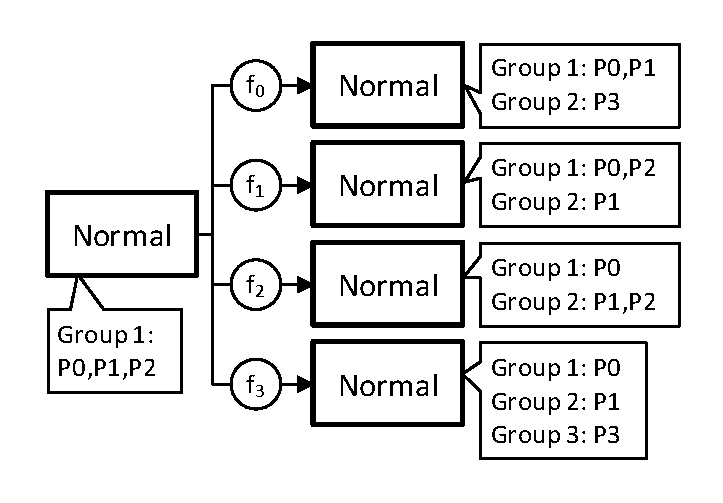
\includegraphics[width=.9\linewidth]{MarkovAYC2.pdf}
\caption{A diagram showing a partial Markov chain for failure detection}
\label{fig:MARKOVAYC}
\end{figure}

Figure 9 illuststrates the model of the failure detection stage of the leader election algorithm.
A set of processes begin in a normal state as part of a group.
The leader sent a query to every member, and every member sent a query to the leader.
If a response was not received in either direction, the process was considered to be unreachable.
If the original message was sent by the leader, the leader removed that member and informed the remaining members.
Otherwise, the member that sent the original message entered a recovery state.

The system remained in the original state as long as all nodes completed their queries and responses.
Let $T_{R}$ be the amount of time allowed for a response, $T_{C}$ be the time between discovery attempts, and $p_{F}$ be the probability that at least one peer failed to complete the exchange.
Based on this, the expected amount of time in the grouped state ($T_{G}$) was
\begin{equation}
\begin{cases}
T_{G} = ( T_{R}+T_{C}  ) / p_{F} & p_{F} > 0 \\
\infty & p_{F} = 0
\end{cases}
\end{equation}
Let $\delta$ equal the exponential parameter of the exponential distribution for the expected time in some set of groups.
The probabilities of each possible transition can then be related to the parameter for that configuration.
Let $p_{i}$ be the probability of transitioning to some set of groups $i$ and let $f_{i}$ be the exponential parameter for the transition to some other configuration:

\begin{equation}
\delta = \sum f_{i} = \sum \delta p_{i} = \frac{1}{T_{G}}
\end{equation}


\subsubsection{Leader Election}
During elections, a highest priority leader (identified by its process id) will
send invites to the other leaders it has identified. If those leaders accept
the highest priority leader's invites, they will reply with an accept message
and forward the invite to their members, if there are any. If the highest
priority process fails to become the leader the next highest will send invites
after a specified interval has passed.

Therefore, the membership of the system can be affected in two ways: election
events which change the size of groups and failure suspicion (via checks) which
decreases the size of groups. Note that elections can decrease the size of
groups as well as increase them: If a round of forwarding invites fails by the
new leader to his original group, the group size could decrease.

When a process is initialized it begins in the ``solo'' state: it is in a group
with itself as the only member. As nodes are discovered by checks, the
processes combine into groups. Groups are not limited by increasing one a time;
they can increase by combined size of the groups of the leader processes.



\begin{figure*}
\centering
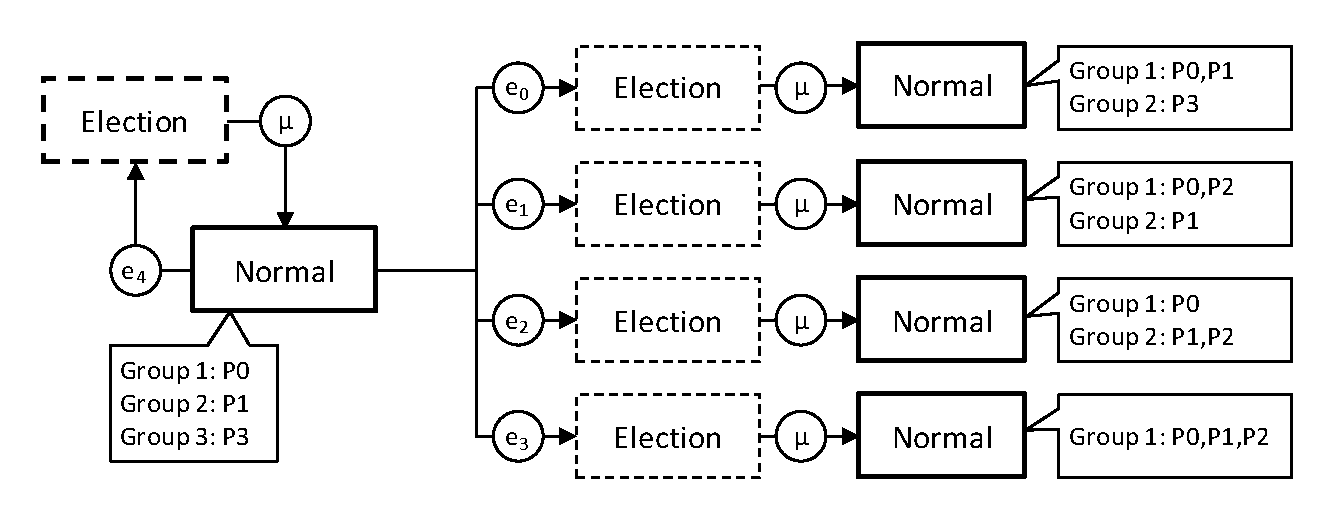
\includegraphics[width=1.0\linewidth]{MarkovElection2.pdf}
\caption{A diagram showing a partial Markov chain for an election}
\label{fig:MARKOVELECTION}
\end{figure*}

A continuous time Markov model of a single election is presented in Figure \ref{fig:MARKOVELECTION}.
A set of leaders begin in a normal state. After some time $T_{D}$ an ``are you coordinator''
message discovers some other peer. $T_{D}$ is a function of the number of discovery
checks which discover no leaders (which in turn is a function of the link reliability). Let
$T_{R}$ be the amount of time allowed for a response, $T_{C}$ be the time between
discovery attempts, and $p_{D}$ is the probability that the exchange discovers a leader.

\begin{equation}
\begin{cases}
T_{D} = ( T_{R}+T_{C} ) / p_{D} & p_{D} > 0 \\
\infty & p_{D} = 0
\end{cases}
\end{equation}

Then, the parameters $e_x$ in Figure \ref{fig:MARKOVELECTION} are a function of $T_{D}$ and $p_{x}$,
the probability an election results in configuration $x$.

\begin{equation}
e_x = \frac{p_{x}}{T_{D}}
\end{equation}

Once a leader has been discovered, the system transitions into an election state, based on the
potential outcome, where the peers hold an election to determine a new configuration. As shown
in Figure \ref{fig:MARKOVELECTION}, an election can either succeed or fail, resulting in a new system
configuration, or each involved process returing to the single member group state.
 
The amount of time that an election takes is fixed before the algorithm is executed. 
Let $T_{E}$ be the mean time it takes to complete any election. Therefore:

\begin{equation}
\mu = \frac{1}{T_{E}}
\end{equation}

\subsubsection{Combined Model}

A combined model combines election and failure detection Markov chain components. Except for the
states where all reachable nodes are in the same group and the states where there are no reachable
leaders each state has a combination of election transitions and failure transitions.                                                        
The combined model is predictive of the overall characteristics of the system. The
time spent in a particular configuration is a function of the $\lambda$'s of all the
events that can cause the system to transition away from a configuration. 

To construct the Markov chain, simulations of individual events are performed. The circumstances
for the events are assumed to be homogeneous: processes only differ by their process id.
Using this assumption, the simulation of events can be broken down into a series of scenarios
that are representative of the events in the system. Since each scenario is independent of other
scenarios, each scenario can be run independently.  Additionally, since the circumstances
are assumed to be homogeneous, scenarios that are similar, such as ones where two processes
swap roles can be simulated only once, and the results can be transformed from one scenario
to another with a simple mapping. This mapping scheme and parallizability helps keep the
state space explosion of the potential states under control.

\section{Model Calibration}

The presented methodology of constructing the model was initially calibrated against the
original two-node case, using a non-real-time version of the DGI codebase. The resulting
Markov chain was processed using SharpE \cite{SHARPE}\cite{SHARPE2} made by Dr. Kishor
Trivedi's group at Duke University, a popular tool for reliability analysis. SharpE measured the reward collected in 600 seconds,
minus the reward that was collected in the first 60 seconds (to emulate that the first
60 seconds were discarded in the experimental runs.) The SharpE results are plotted along
with the experimental results in Figures \ref{fig:COMPARE-SUC-2NODE-100} and \ref{fig:COMPARE-SUC-2NODE-200}.

\begin{figure}[!h]
\centering
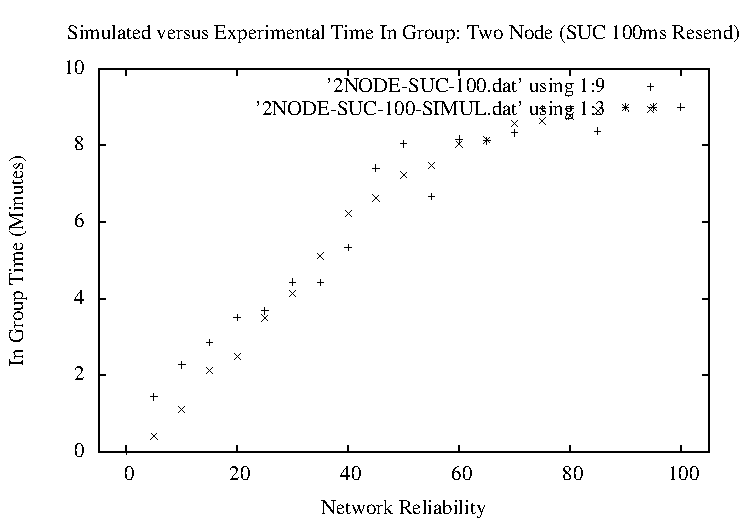
\includegraphics[width=1.0\linewidth]{2NODE-SUC-100-COMPARE.pdf}
\caption{Comparison of in group time as collected from the experimental platform and the simulator (1 tick offset between processes).}
\label{fig:COMPARE-SUC-2NODE-100}
\end{figure}


\begin{figure}[!h]
\centering
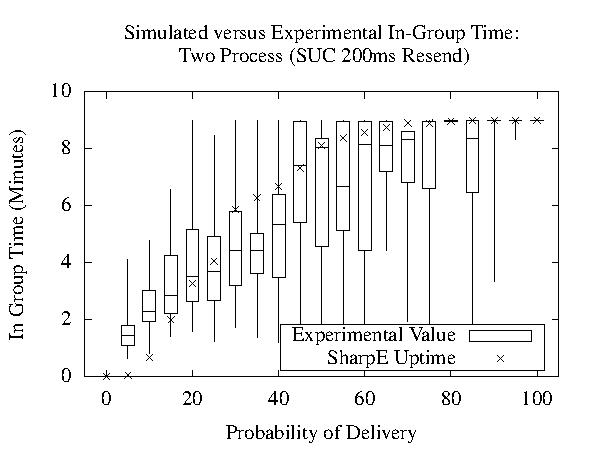
\includegraphics[width=1.0\linewidth]{2NODE-SUC-200-COMPARE.pdf}

\caption{Comparison of in group time as collected from the experimental platform and the simulator (2 tick offset between processes).}
\label{fig:COMPARE-SUC-2NODE-200}
\end{figure}

The race condition between processes during an election is a consideration in the original
leader election algorithm, and is an additional factor here. The simulator provided a parameter
to allow the operator to select how closely synchronized the peers were (the time difference
between when each of them would search for leaders.) The exchange of messages, particularly
during an election had a tendency to synchronize nodes during elections, and so the nodes could
synchronize even if they did not initially begin in a synchronized state. As a result, the
simulation results aligned best for the 100ms resend case with 1 ticks (Approximately 100ms
difference in synchronization between processes) and 2 ticks (Approximately 400ms) in the 200ms
resend case.

Models fit to the non-real-time code in groups larger than 2 processes did not fit well.
This is presumed to be a combination of several factors. The suspected major source of fault
included the structure of the chain, which naturally assumes that all processes enter the
election state a roughly the same time, which is not typically true for any number of processes
greater than 2. Additionally, the simulator could only assume that the synchronization between
processes was mostly fixed, which was not the case in the larger configurations, since the
coincidental synchronization that occurred in the two node case was suppressed by the increased
number of peers. Furthermore, an issue with SharpE was discovered that prevented the
particular structure of the chains produced from being handled correctly. To circumvent that,
issue, SharpE was replaced by a random-walker which generates exponentially distributed numbers
and follows the paths of the chain, across several hundred trials, in order to collect time in group data for
models which SharpE cannot process.

The structure of the Markov Chain, which assumed that processes enter the election state
mostly simultaneously was an appropriate assumption for the real-time system, since the
round-robin scheduler synchronizes when processes run their group management modules. The
simulator was set to assume that the synchronization between processes was very tight, and
new experimental data was collected for the 4 node, transient partition case. The collected
data is overlaid with the results from the random walker in Figures \ref{fig:COMPARE-SUC-TRANS-RT-128} and \ref{fig:COMPARE-SUC-TRANS-RT-64}.

\begin{figure}[!h]
\centering
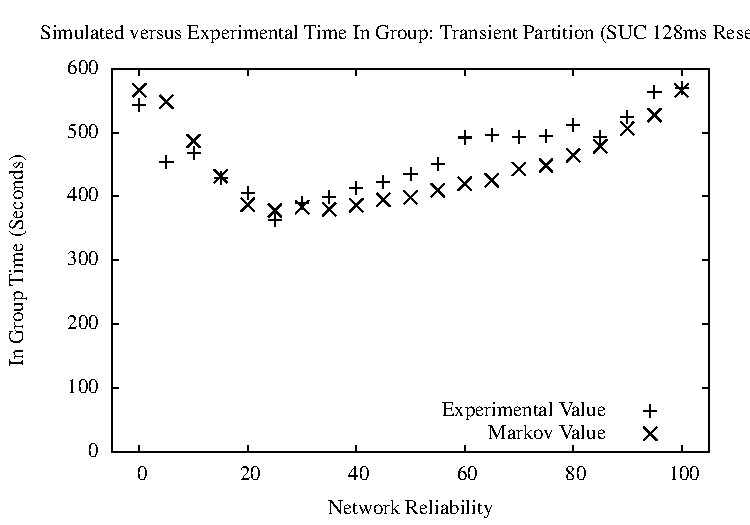
\includegraphics[width=1.0\linewidth]{TRANS-RT-SUC-128-COMPARE.pdf}

\caption{Comparison of in group time as collected from the experimental platform and the time in group from the equivalent Markov chain (128ms between resends).}
\label{fig:COMPARE-SUC-TRANS-RT-128}
\end{figure}

\begin{figure}[!h]
\centering
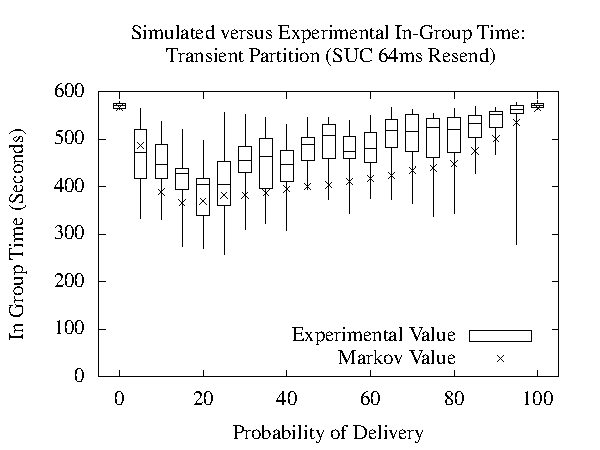
\includegraphics[width=1.0\linewidth]{TRANS-RT-SUC-64-COMPARE.pdf}

\caption{Comparison of in group time as collected from the experimental platform and the time in group from the equivalent Markov chain (64ms between resends).}
\label{fig:COMPARE-SUC-TRANS-RT-64}
\end{figure}

As a measure of the strength of the model, the correlation between the predicted value was compared.
The average error was also computed for each of the samples taken. This information is presented in
Table \ref{tab:STAT-DATA}.

\begin{table}
% increase table row spacing, adjust to taste
\caption{Error and correlation of experimental data and Markov chain predictions}
\label{tab:STAT-DATA}
\centering
% Some packages, such as MDW tools, offer better commands for making tables
% than the plain LaTeX2e tabular which is used here.
\begin{tabular}{|c||c|c|c|} 
\hline
Resend & Correlation & Error \\ \hline
128 & 0.7656 & 11.61\% \\ \hline
64 & 0.8604 & 11.70\% \\ \hline 
\end{tabular}
\end{table}

\section{Conclusion}

This work presented a new approach for predicting the behavior of a real-time
distributed system under omission failure conditions. By using a continuous time
Markov chain, a variety of insights can be gathered about the system, including
observations such as how long a particular configuration will be stable for, 
and the behavior of the system in the long run.  The Markov results will be used
 to make better real time schedules to better react to the network faults we
plan on introducing to our testbeds. For example, if migrations are failing
and a sufficient number of migrations can cause the physical system to fail,
the scheduler may need to behave in a manner that limits the number of failed
migrations that can occur before group reconfigures. This work is a stepping
stone towards designing a real-time schedule that manages the system correctly
when there are cyber faults. Schedules and behavior can be designed around how
the system behaves on its worst days. This work also allows these schedule designs
and evaluations to be completed much more quickly than they could be by running
the system for long periods of time. Therefore results from the test bed, combined
with results the models yield schedules that improve the stability of the
system during cyber faults.




